\documentclass[a4paper,12pt]{article}
\usepackage{geometry}
\geometry{left=3cm,right=3cm,top=3cm,bottom=3cm,footskip=2cm}
\usepackage{setspace}	
\linespread{1.3}

\usepackage{lmodern}
\usepackage{amssymb,amsmath}
%\usepackage{ifxetex,ifluatex}
%\usepackage{fixltx2e} % provides \textsubscript
\usepackage[T1]{fontenc}
\usepackage[utf8]{inputenc}
\usepackage{eurosym}
%\usepackage{natbib}
%\bibliographystyle{plainnat}
%\usepackage{biblatex}
%\bibliography{}
\usepackage{listings}
%Allow degree escape in listings
\usepackage{gensymb}
\lstnewenvironment{code}{\lstset{language=Haskell,basicstyle=\small\ttfamily}}{}
\usepackage{color}
\usepackage{fancyvrb}
\newcommand{\VerbBar}{|}
\newcommand{\VERB}{\Verb[commandchars=\\\{\}]}
\DefineVerbatimEnvironment{Highlighting}{Verbatim}{commandchars=\\\{\}}
% Add ',fontsize=\small' for more characters per line
\newenvironment{Shaded}{}{}
\newcommand{\KeywordTok}[1]{\textcolor[rgb]{0.00,0.44,0.13}{\textbf{{#1}}}}
\newcommand{\DataTypeTok}[1]{\textcolor[rgb]{0.56,0.13,0.00}{{#1}}}
\newcommand{\DecValTok}[1]{\textcolor[rgb]{0.25,0.63,0.44}{{#1}}}
\newcommand{\BaseNTok}[1]{\textcolor[rgb]{0.25,0.63,0.44}{{#1}}}
\newcommand{\FloatTok}[1]{\textcolor[rgb]{0.25,0.63,0.44}{{#1}}}
\newcommand{\ConstantTok}[1]{\textcolor[rgb]{0.53,0.00,0.00}{{#1}}}
\newcommand{\CharTok}[1]{\textcolor[rgb]{0.25,0.44,0.63}{{#1}}}
\newcommand{\SpecialCharTok}[1]{\textcolor[rgb]{0.25,0.44,0.63}{{#1}}}
\newcommand{\StringTok}[1]{\textcolor[rgb]{0.25,0.44,0.63}{{#1}}}
\newcommand{\VerbatimStringTok}[1]{\textcolor[rgb]{0.25,0.44,0.63}{{#1}}}
\newcommand{\SpecialStringTok}[1]{\textcolor[rgb]{0.73,0.40,0.53}{{#1}}}
\newcommand{\ImportTok}[1]{{#1}}
\newcommand{\CommentTok}[1]{\textcolor[rgb]{0.38,0.63,0.69}{\textit{{#1}}}}
\newcommand{\DocumentationTok}[1]{\textcolor[rgb]{0.73,0.13,0.13}{\textit{{#1}}}}
\newcommand{\AnnotationTok}[1]{\textcolor[rgb]{0.38,0.63,0.69}{\textbf{\textit{{#1}}}}}
\newcommand{\CommentVarTok}[1]{\textcolor[rgb]{0.38,0.63,0.69}{\textbf{\textit{{#1}}}}}
\newcommand{\OtherTok}[1]{\textcolor[rgb]{0.00,0.44,0.13}{{#1}}}
\newcommand{\FunctionTok}[1]{\textcolor[rgb]{0.02,0.16,0.49}{{#1}}}
\newcommand{\VariableTok}[1]{\textcolor[rgb]{0.10,0.09,0.49}{{#1}}}
\newcommand{\ControlFlowTok}[1]{\textcolor[rgb]{0.00,0.44,0.13}{\textbf{{#1}}}}
\newcommand{\OperatorTok}[1]{\textcolor[rgb]{0.40,0.40,0.40}{{#1}}}
\newcommand{\BuiltInTok}[1]{{#1}}
\newcommand{\ExtensionTok}[1]{{#1}}
\newcommand{\PreprocessorTok}[1]{\textcolor[rgb]{0.74,0.48,0.00}{{#1}}}
\newcommand{\AttributeTok}[1]{\textcolor[rgb]{0.49,0.56,0.16}{{#1}}}
\newcommand{\RegionMarkerTok}[1]{{#1}}
\newcommand{\InformationTok}[1]{\textcolor[rgb]{0.38,0.63,0.69}{\textbf{\textit{{#1}}}}}
\newcommand{\WarningTok}[1]{\textcolor[rgb]{0.38,0.63,0.69}{\textbf{\textit{{#1}}}}}
\newcommand{\AlertTok}[1]{\textcolor[rgb]{1.00,0.00,0.00}{\textbf{{#1}}}}
\newcommand{\ErrorTok}[1]{\textcolor[rgb]{1.00,0.00,0.00}{\textbf{{#1}}}}
\newcommand{\NormalTok}[1]{{#1}}
\usepackage{longtable,booktabs}
\usepackage{graphicx}
\makeatletter
\def\maxwidth{\ifdim\Gin@nat@width>\linewidth\linewidth\else\Gin@nat@width\fi}
\def\maxheight{\ifdim\Gin@nat@height>\textheight\textheight\else\Gin@nat@height\fi}
\makeatother
% Scale images if necessary, so that they will not overflow the page
% margins by default, and it is still possible to overwrite the defaults
% using explicit options in \includegraphics[width, height, ...]{}
\setkeys{Gin}{width=\maxwidth,height=\maxheight,keepaspectratio}
\usepackage[unicode=true]{hyperref}
\hypersetup{breaklinks=true,
            bookmarks=true,
            pdfauthor=Esteban Munoz,
            pdftitle=Guidelines Energy-ADE,
            colorlinks=true,
            citecolor=blue,
            urlcolor=blue,
            linkcolor=magenta,
            pdfborder={0 0 0}}
\urlstyle{same}  % don't use monospace font for urls
% Make links footnotes instead of hotlinks:
\renewcommand{\href}[2]{#2\footnote{\url{#1}}}
\setlength{\parindent}{0pt}
\setlength{\parskip}{6pt plus 2pt minus 1pt}
\setlength{\emergencystretch}{3em}  % prevent overfull lines
%%\setcounter{secnumdepth}{0}
%
%% Reformat Sections
\let\stdsection\section%
\renewcommand\section{\newpage\stdsection}

%% Title Page
\usepackage{fancyhdr}
\pagestyle{fancy}
\fancyhf{}

%% Normal page
\fancypagestyle{normalpage}{%
\fancyhf{}
\rhead{%
    \begin{footnotesize}
        ADE Energy Core
    \end{footnotesize}
}
\lfoot{%
    \begin{footnotesize}
        {}
    \end{footnotesize}
    }
\rfoot{%
    \begin{footnotesize}
        \thepage%
    \end{footnotesize}
}
\renewcommand{\headrulewidth}{0pt} % remove lines as well
\renewcommand{\footrulewidth}{0pt}
\renewcommand{\headwidth}{17cm}
}

%% Title Page
\fancypagestyle{titlepage}{%
\fancyhf{}
% The title page has different margins 
\renewcommand{\headrulewidth}{0pt} % remove lines as well
\renewcommand{\footrulewidth}{0pt}
}

\pagestyle{titlepage}
\usepackage{color}
\definecolor{lightgray}{gray}{0.60}
%% Maketitle
\renewcommand\maketitle{%
\sffamily
\begin{flushright}

\includegraphics[width=4cm]{./fig/logo.png}
\end{flushright}
    \thispagestyle{titlepage}
    \vspace{3.4cm}
    {\noindent \textcolor{lightgray}{Draft Guidelines - Energy ADE version 0.6} \par}
    \vspace{0.3cm}
    {\noindent \large \bfseries CityGML Energy Application Domain Extension \par}
    \vspace{0.7cm}
    {\noindent In collaboration with OGC and SIG 3D \par}
    \vspace{0.7cm}
    {\noindent \textcolor{lightgray}{\today} \par}
\newpage
\begin{flushleft}
\begin{tabular}{lll}
    \toprule
    \textbf{Revision updates} & \textbf{When} & \textbf{Who}\\
    \midrule
    Basis version &
    03.08.2015 &
    RN
\\
    Markdown export &
    22.10.2015 &
    EM
%    Basis version\\Markdown export 
    \\
    \bottomrule
\end{tabular}
\end{flushleft}
\textbf{Authors:}\\
{\noindent \normalsize \normalfont%
Romain Nouvel (RN)\\Marcel Bruse\\Olivier Tournaire\\Esteban Mu\(\~n\)oz (EM)\\\dots}
\par
\vspace{0.3cm}
\textbf{Consortium participating institutes:}
\begin{itemize}
    \itemsep-1.3em
    \item University of Applied Sciences Stuttgart, Germany\\\item Technische Universität München, Germany\\\item Karlsruhe Institute für Technologie, Germany\\\item European Institute for Energy Research, Germany\\\item RWTH Aachen University / E.ON Energy Research Center, Germany\\\item HafenCityUniversität Hamburg, Germany\\\item Ecole Polytechnique Fédérale de Lausanne, Switzerland\\\item Centre Scientifique et Technique du Batiment, France\\\item Electricité de France, France\\\item Sinergis, Italy\\\item M.O.S.S Computer Grafik Système, Germany
\end{itemize}
\newpage
}

\begin{document}
\pagestyle{titlepage}
\maketitle
\pagestyle{normalpage}
\begin{abstract}
The Application Domain Extension (ADE) Energy detailed in this
documentation defines a standardized data model based on CityGML format
for urban energy analyses, aiming to be a reference exchange data format
between different urban modelling tools and expert databases.

It has been developed since May 2014 by an international consortium of
urban energy simulation developers and users (University of Applied
Sciences Stuttgart, Technische Universität München, Karlsruhe Institute
für Technologie, RWTH Aachen University / E.ON Energy Research Center,
HafenCity Universität Hamburg, European Institute for Energy Research,
Ecole Polytechnique Fédérale de Lausanne, Centre Scientifique et
Technique du Batiment, Electricité de France, Sinergis and M.O.S.S
Computer Grafik Systeme).
\end{abstract}
\newpage
\pagestyle{normalpage}


\hypersetup{linkcolor=black}
\tableofcontents
\newpage
\section{Overview of the Application Domain Extension
Energy}\label{overview-of-the-application-domain-extension-energy}

The CityGML Energy ADE aims at extending the CityGML standard with
energy-related entities necessary to lead energy analyses at urban
scale.

Following the philosophy of CityGML, this Energy ADE aims to be
flexible, in terms of compatibility with different data qualities,
levels of details, and urban energy models complexities (from monthly
energy balance of ISO 13790, to sub-hourly dynamic simulation of
softwares like CitySim or EnergyPlus). It takes into consideration the
INSPIRE Directive of the European Parliament, as well as the recent US
Building Energy Data Exchange Specification (BEDES).

Its structure is thought of as modular; some of its modules can be
potentially used and extended for other applications (e.g.~module
Occupancy for socio-economics, module Materials for acoustics or
statics, module Metadata and Scenarios for every urban analysis).

\section{Building Physics Module}\label{building-physics-module}

This central module of the Energy ADE contains the thermal building
objects required for the building energy modelling (e.g.
\texttt{ThermalZone}, \texttt{ThermalBoundary},
\texttt{ThermalComponent}). These thermal building objects are linked to
the CityGML building objects through its \texttt{\_AbstractBuilding},
\texttt{\_BoundarySurface} and \texttt{\_Opening} classes.

\subsection{Building, zones and
boundaries}\label{building-zones-and-boundaries}

\begin{figure}[htbp]
\centering
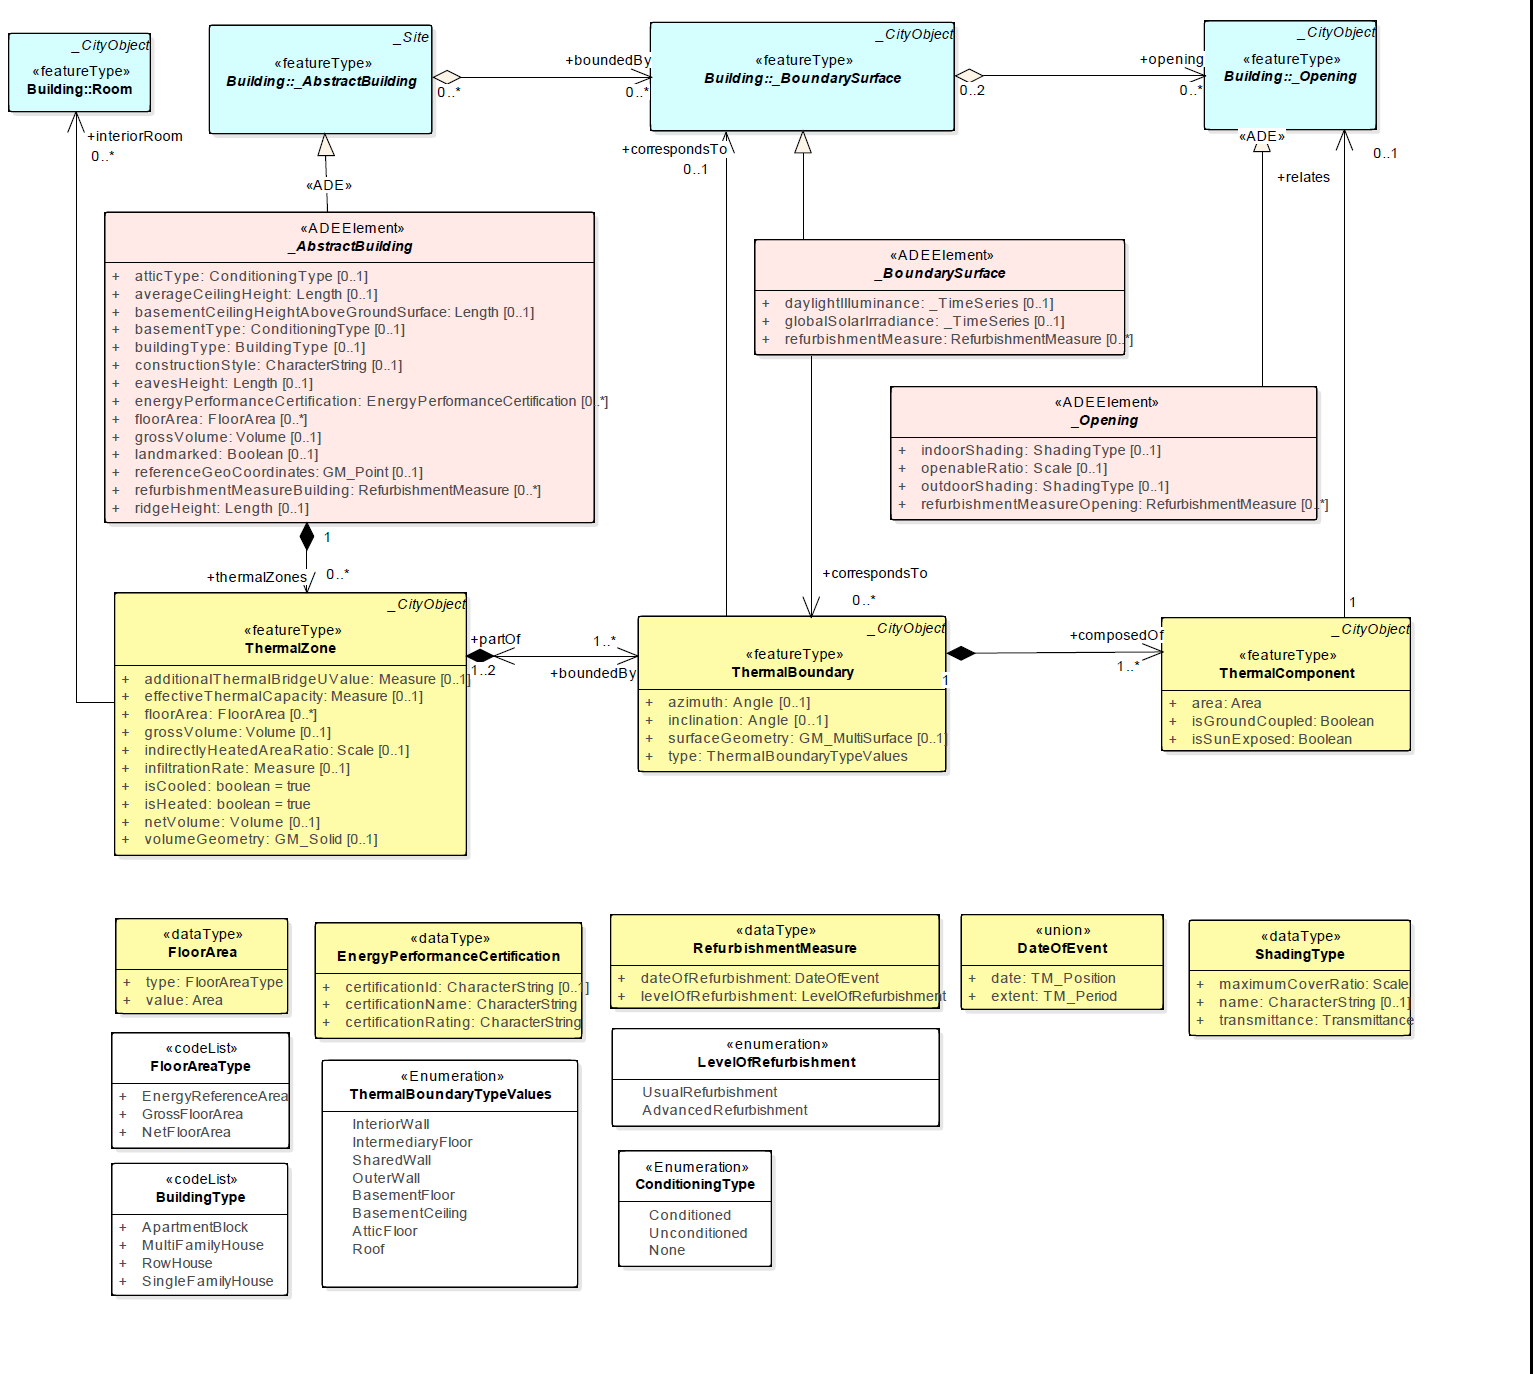
\includegraphics{fig/class_geometry.png}
\caption{Class diagram of Building Physics Module}
\end{figure}

\subsubsection{ThermalZone}\label{thermalzone}

Zone of a building which serves as space unit for building
heating/cooling simulations, a thermal zone is considered as isothermal.
It is a semantic object, with an optional geometry, which may be or not
related to a geometric entity (\texttt{gml:Building},
\texttt{gml:BuildingPart}, \texttt{gml:Room} etc.).

This class inherits from \texttt{\_CityObject}, and may therefore be
associated to 1 or more \texttt{EnergyDemand} objects (see module Energy
systems). For the requirement of the building heating/cooling
simulations, the \texttt{ThermalZone} must be related to one or more
\texttt{UsageZone} (see Occupancy Module).

\subsubsection{ThermalBoundary}\label{thermalboundary}

Quasi-coplanar surface delimiting thermal zones. It represents the
physical relationship between two thermal zones (defining the thermal
zones adjacency) or a thermal zone and the building surrounding.

It is a semantic object, with an optional geometry. It may be linked to
the \texttt{gml:BoundarySurface} (through the
\texttt{ADE:\_BoundarySurface}) when possible, but not necessary
(e.g.~cellar ceiling or top storey ceiling in the case of CityGML LoD1
to LoD3).

While separating two thermal zones, its optional geometry corresponds to
the middle of the internal/shared wall. While separating a thermal zone
from the building surrounding, its optional geometry corresponds to the
external surface of the outer wall/roof/basement floor. The following
figure represents these different cases in a building side section,
relating the Energy ADE Objects \texttt{ThermalZone} and
\texttt{ThermalBoundary} to the CityGML objects \texttt{Room} (could be
also \texttt{Building} or \texttt{BuildingPart}) respectively
\texttt{WallSurface}, \texttt{RoofSurface}, \texttt{FloorSurface},
\texttt{CeilingSurface} and \texttt{InteriorWallSurface}.

\begin{figure}[htbp]
\centering
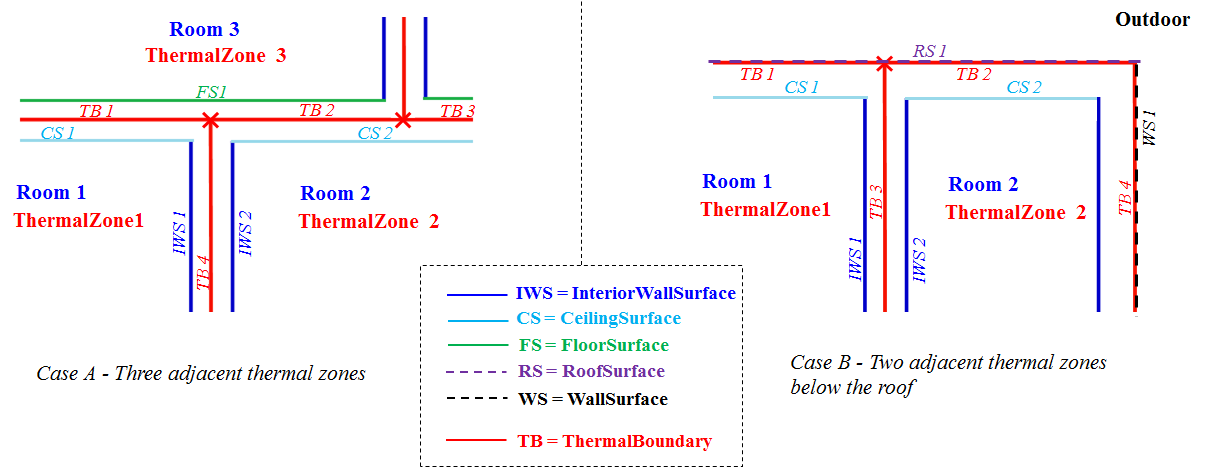
\includegraphics{fig/ThermalZoneAdjacency.png}
\caption{Schema of adjacent thermal zones}
\end{figure}

\subsubsection{ThermalComponent}\label{thermalcomponent}

Part of the thermal boundary corresponding to a homogeneous construction
component (e.g.~windows, wall, insulated part of a wall etc.).

This class inherits from \texttt{\_CityObject}, which allows him to be
associated to a Construction Object (see module Construction and
Material).

\subsubsection{\_AbstractBuilding}\label{abstractbuilding}

Extension of CityGML object \texttt{\_AbstractBuilding} in Application
Domain Extension Energy.

\subsubsection{\_BoundarySurface}\label{boundarysurface}

Extension of CityGML object \texttt{\_BoundarySurface} in Application
Domain Extension Energy.

Even empty, this subtype is necessary for the connection of the ADE
Energy to the CityGML, since a bi-directional associations to the
existing definitions is added.

\subsubsection{\_Opening}\label{opening}

Extension of CityGML object \texttt{\_Opening} in Application Domain
Extension Energy. Openings may have an indoor and an outdoor shading
system. They are further defined by an openable ratio.

\subsection{Solar irradiances and
Daylighting}\label{solar-irradiances-and-daylighting}

To realize solar and daylight potential studies, the Energy ADE enables
to store the incident global solar irradiances, respectively the
daylight illuminances available on each outside boundary surface of the
buildings.

Both \texttt{globalSolarIrradiance} and \texttt{daylightIlluminance} are
attributes of the object \texttt{\_BoundarySurface}, of type
\texttt{\_TimeSeries} (see details in Temporal Data Module).

\subsubsection{globalSolarIrradiance}\label{globalsolarirradiance}

It is the sum of the direct, diffuse and reflected irradiance incident
on a outside boundary surface. Its unit of measure is the Watt per sqm
(\(W/m^2\)). These values are typically used as source terms for the
thermal calculations within the buildings (more precisely the
\texttt{\_ThermalZone}), but also for the calculation of the energy
producted by the solar systems (photovoltaic and solar thermal panels).

\subsubsection{daylightIlluminance}\label{daylightilluminance}

It is the sum of the direct, diffuse and reflected solar illuminance
incident on a outside boundary surface. Its unit of measure is the Lux
(\(lx\)). These values are typically used for outside and inside
daylighting study, as well as the calculation of the energy consumptions
of lighting systems required to reach the room illuminance threshold
when the daylight illuminance is not enough.

\section{Temporal Data Module}\label{temporal-data-module}

\subsection{Time Series}\label{time-series}

\begin{figure}[htbp]
\centering
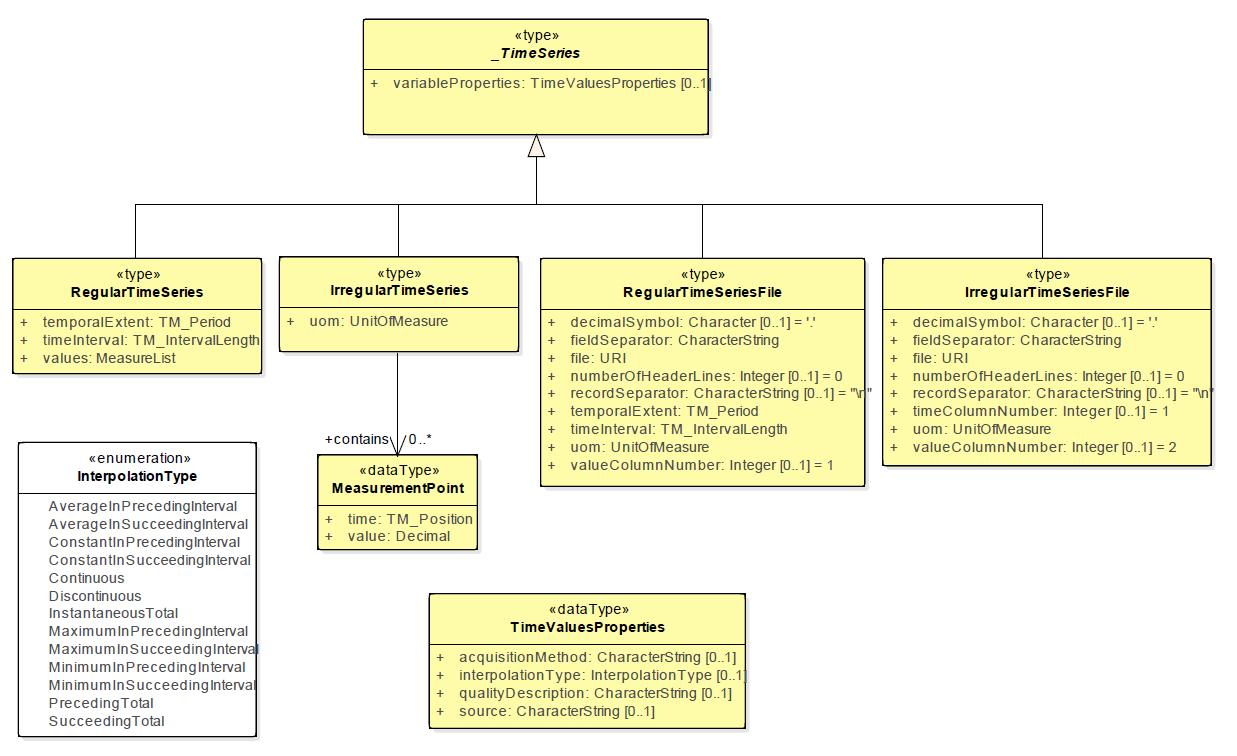
\includegraphics{fig/class_time.png}
\caption{Class diagram of ADE Energy Core - Time Series}
\end{figure}

Time series are homogeneous list of time-depending values. They are used
in the Energy ADE to store energy amount or schedule for instance. As
non-domain specific feature, they is planned to be integrated in the
CityGML 3.0.

They have common properties specified in the type

\subsubsection{TimeValuesProperties}\label{timevaluesproperties}

These properties are the variable label, the variable unit of measure
(\emph{uom}), the interpolation type (based on the
\href{http://def.seegrid.csiro.au/sissvoc/ogc-def/resource?uri=http://www.opengis.net/def/waterml/2.0/interpolationType/}{WaterML
ADE}) and some data acquisition information like the data source, the
acquisition method and the quality description.

Time Series can be either regular or irregular.

\textbf{RegularTimeSeries} contain \texttt{values} generated at
regularly spaced interval of time (\texttt{timeInterval}), over a given
\texttt{temporalExtent} (= start, end and duration time). They are
relevant for instance to store automatically acquired data or
hourly/daily/monthly simulation results.

In \textbf{IrregularTimeSeries}, the data in the time series follows
also a temporal sequence, but the measurement points might not happen at
a regular time interval\footnote{\href{http://www-01.ibm.com/support/knowledgecenter/SSCRJU_3.0.0/com.ibm.swg.im.infosphere.streams.timeseries-toolkit.doc/doc/timeseries-regular.html}{IBM
  knowledge Center}}. Therefore, each value must be associated with a
data or time.

\subsection{Schedules}\label{schedules}

\begin{figure}[htbp]
\centering
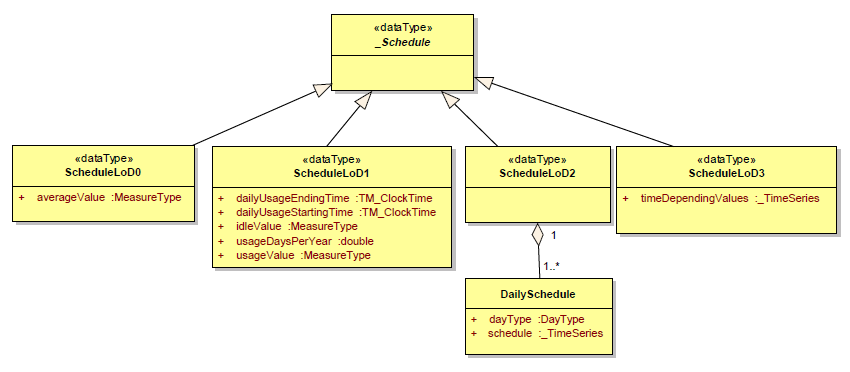
\includegraphics{fig/class_schedules.png}
\caption{Class diagram of ADE Energy Core - Schedules}
\end{figure}

The type Schedule is used in the Energy ADE for different kinds of
schedules and variables, including heating/cooling schedules (set-point
temperatures), ventilation schedules (mechanical air change rate) and
occupancy rate.

Schedules may be modelled with 4 ``semantic levels of details''
depending on the available information and the application.

\subsubsection{ConstantValueSchedule}\label{constantvalueschedule}

Most basic level of detail, it corresponds to a constant value,
generally corresponding to the average parameter value.

\begin{Shaded}
\begin{Highlighting}[]
\CommentTok{<!--Example of the cooling schedule of a residential building:-->}
\KeywordTok{<energy:coolingSchedule>}
    \KeywordTok{<energy:ConstantValueSchedule}\ErrorTok{*}\KeywordTok{>}
        \KeywordTok{<energy:averageValue}\OtherTok{ uom=}\StringTok{"\degree{C}"}\KeywordTok{>}\NormalTok{26}\KeywordTok{</energy:averageValue>}
    \KeywordTok{</energy:ConstantValueSchedule}\ErrorTok{*}\KeywordTok{>}
\KeywordTok{</energy:coolingSchedule>}
\end{Highlighting}
\end{Shaded}

\subsubsection{DualValueSchedule}\label{dualvalueschedule}

Two-state schedule, specified by a usage value defined for usage times,
and an idle value outside this temporal boundaries. Information about
the approximate number of usage days per year and usage hours per usage
days are also defined.

This schedule complies in particular with the data requirements of the
codes and norms describing the monthly energy balance (DIN 18599-2, ISO
13790).

\begin{Shaded}
\begin{Highlighting}[]
\CommentTok{<!--Example of the heating schedule of a residential building:-->}
\KeywordTok{<energy:heatingSchedules>}
    \KeywordTok{<energy:DualValueSchedule>}
        \KeywordTok{<energy:usageValue}\OtherTok{ uom=}\StringTok{"\degree{C}"}\KeywordTok{>}\NormalTok{20}\KeywordTok{</energy:usageValue>}
        \KeywordTok{<energy:idleValue}\OtherTok{ uom=}\StringTok{"\degree{C}"}\KeywordTok{>}\NormalTok{16}\KeywordTok{</energy:idleValue>}
        \KeywordTok{<energy:usageHoursPerDay}\OtherTok{ uom=}\StringTok{""}\KeywordTok{>}\NormalTok{17}\KeywordTok{</energy:usageHoursPerDay>}
        \KeywordTok{<energy:usageDaysPerYear}\OtherTok{ uom=}\StringTok{""}\KeywordTok{>}\NormalTok{365}\KeywordTok{</energy:usageDaysPerYeary>}
    \KeywordTok{</energy:DualValueSchedule>}
\KeywordTok{</energy:heatingSchedules>}
\end{Highlighting}
\end{Shaded}

\subsubsection{DailyPatternSchedule}\label{dailypatternschedule}

Detailed schedule composed of daily schedules associated to recurrent
day types (weekday, weekend etc.). These daily schedules are Time Series
as described above.

\subsubsection{TimeSeriesSchedule}\label{timeseriesschedule}

Most detailed schedule corresponding to a Time series as described
above.

\section{Construction and Material
Module}\label{construction-and-material-module}

\begin{figure}[htbp]
\centering
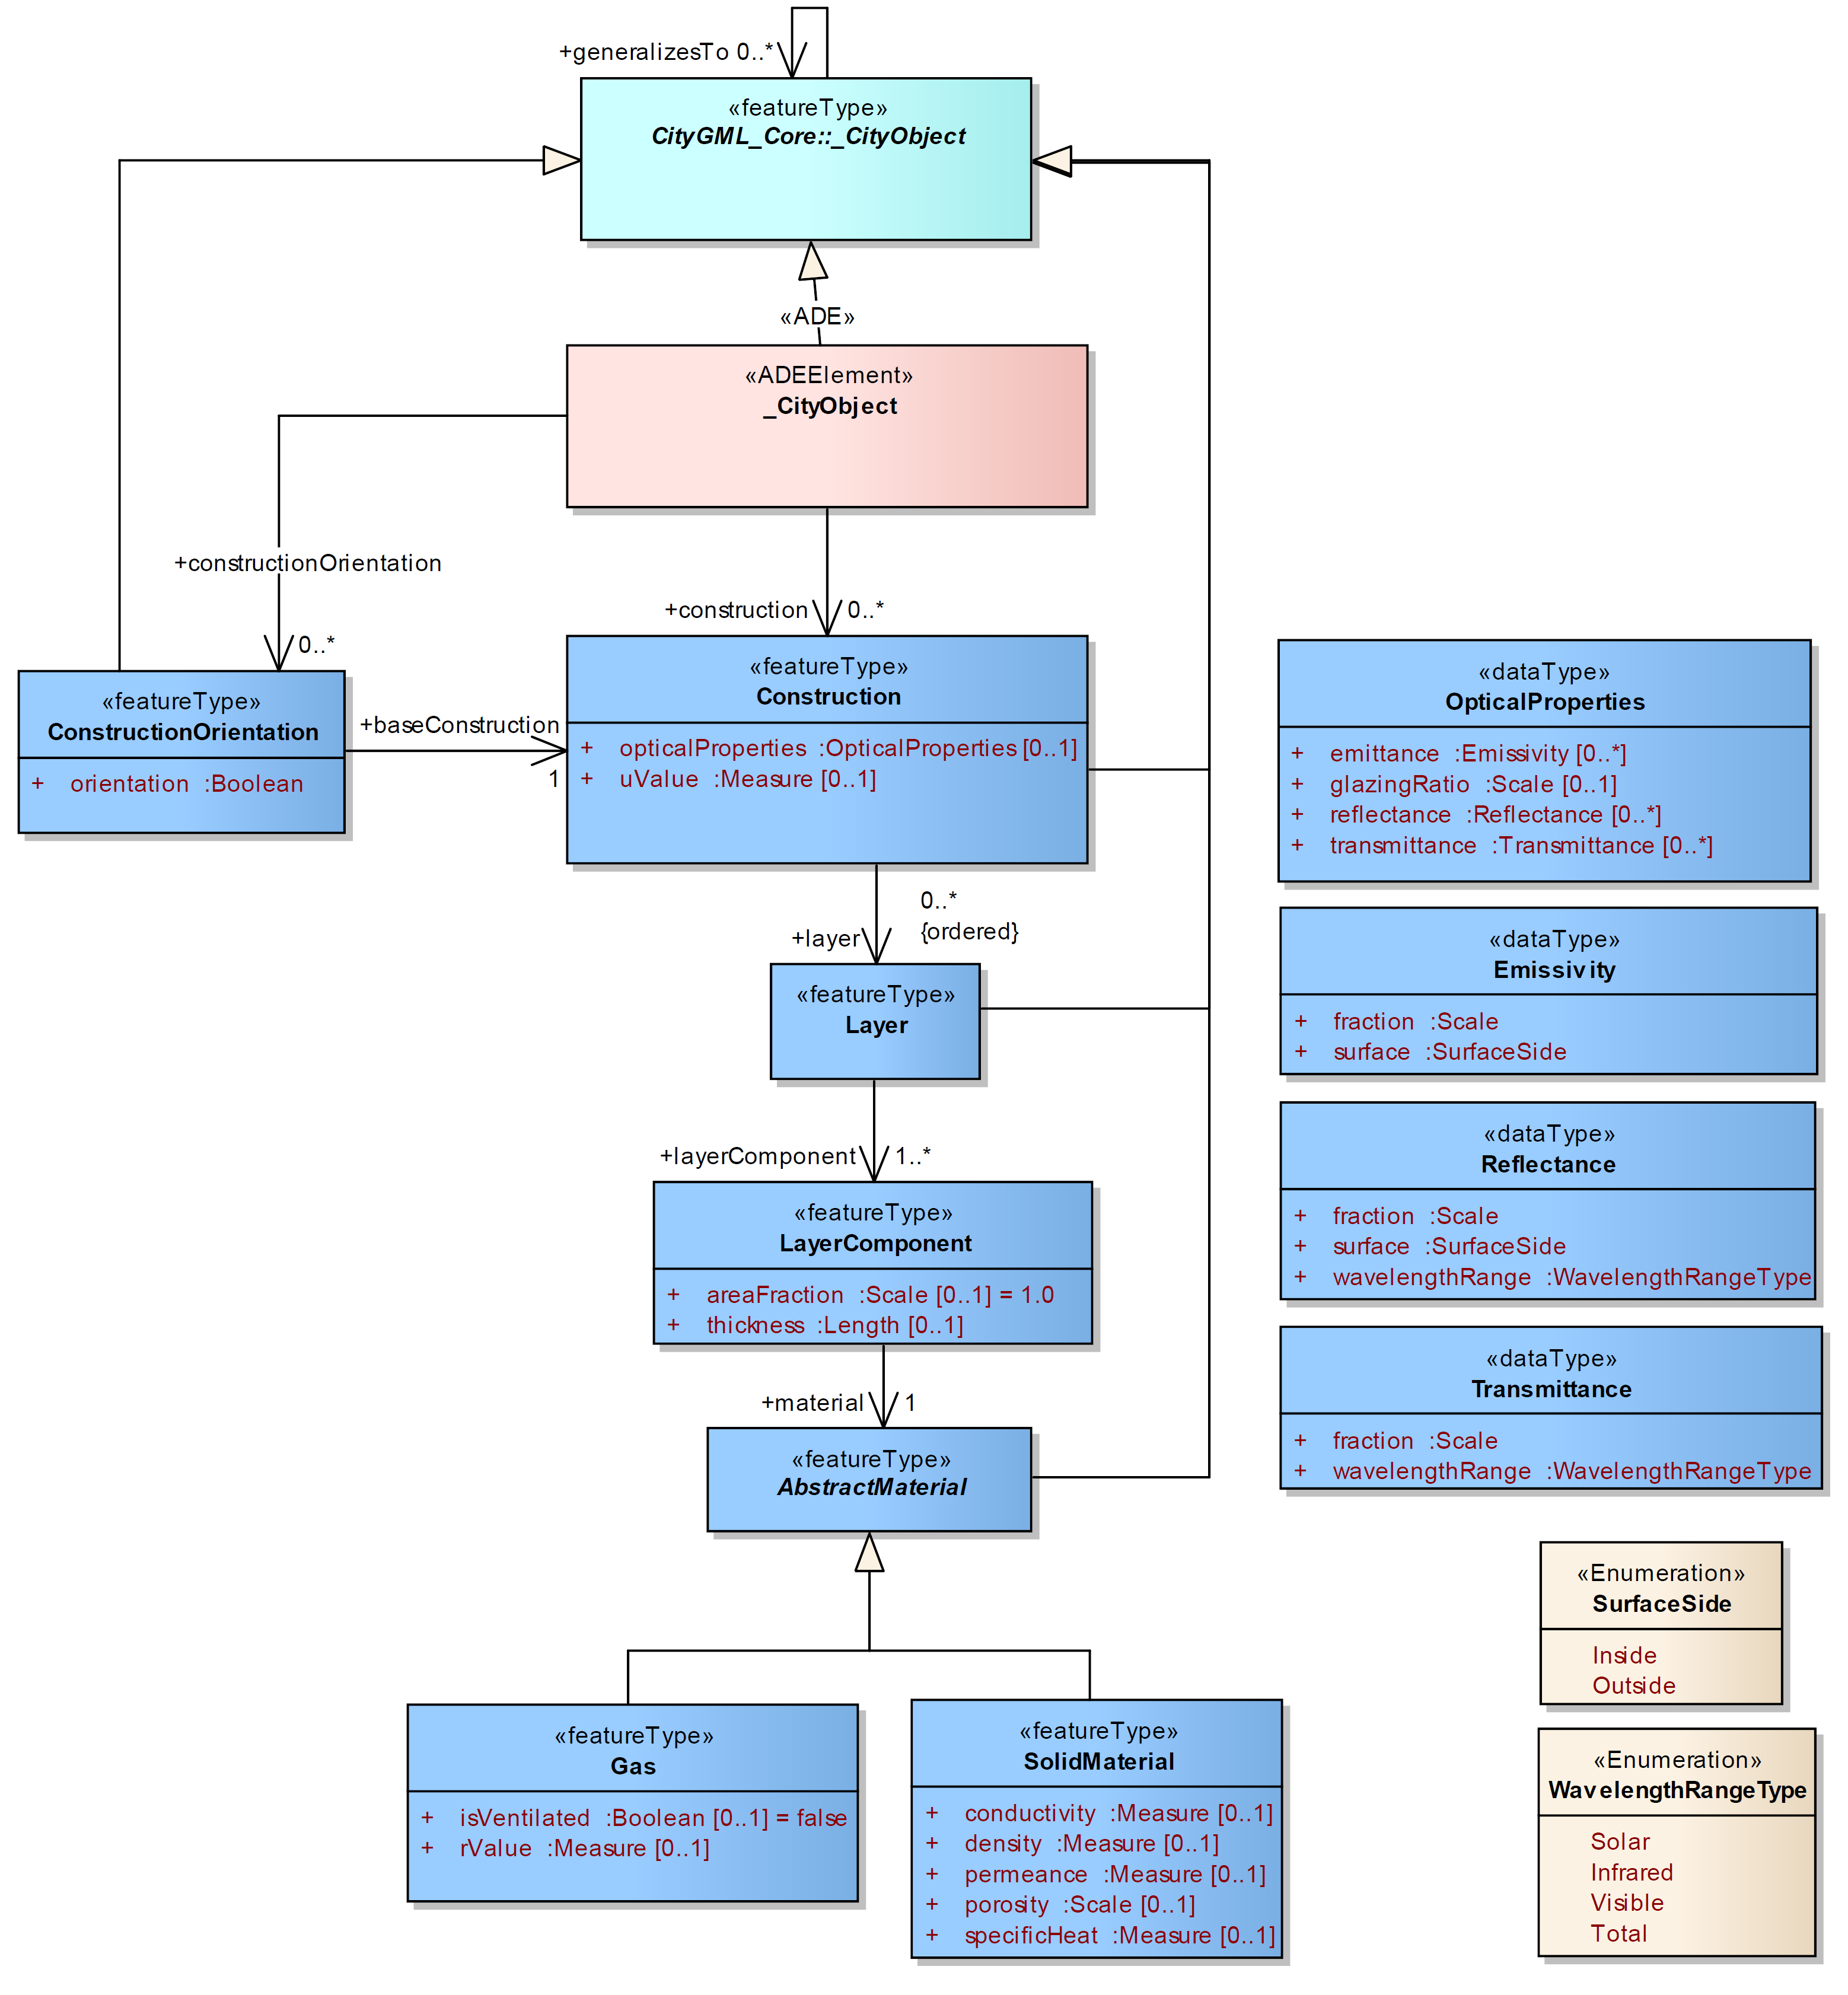
\includegraphics{fig/class_construction.png}
\caption{Class diagram of Construction Module}
\end{figure}

The Construction and Material is a module of the ADE Energy, which
contains the physical characterization of the boundary surfaces, surface
components and even whole building (and potentially all the objects
which inherits of \texttt{\_CityObject}).

It may be extended for multi-field analysis (statics, acoustics etc.).

\subsection{Construction and layers}\label{construction-and-layers}

\subsubsection{Construction}\label{construction}

Physical characterisation of building envelop or intern room partition
(e.g.~wall, roof, openings), it may be specified as an ordered
combination of layers.

In the Energy ADE, the object Construction aims to be linked to the
\texttt{\_ThermalComponents}, in order to defined the physical
parameters of a walls, roofs of windows, for a space heating/cooling
calculation. However, it may possibly be linked to any
\texttt{\_CityObject} for other purposes, in particular to
\texttt{gml:\_BoundarySurface}, \texttt{gml:\_Opening} or even
\texttt{\_AbstractBuilding}.

{[}XML code example{]}

\subsubsection{ConstructionOrientation}\label{constructionorientation}

Class defining the orientation convention of the Construction, it means
the order of the layers. A same Construction, common to different zones
or buildings, will be orientated in two different directions for
instance.

\subsubsection{Layer}\label{layer}

Combination of one of more materials, referenced via a layer component.

It inherits from \texttt{\_CityObject}.

\subsubsection{LayerComponent}\label{layercomponent}

Homogeneous part of a layer, covering a given fraction
(\texttt{areaFraction}) of the layer.

\subsection{Materials}\label{materials}

\subsubsection{AbstractMaterial}\label{abstractmaterial}

Abstract superclass for all Material classes. A Material is a
homogeneous substance. We distinguish solid materials (with mass) from
gas (without mass).

\subsubsection{SolidMaterial}\label{solidmaterial}

Class of the materials which have a mass and a heat capacity.

\subsubsection{Gas}\label{gas}

Class of the material whose mass and heat capacity are neglectable in
comparison with \texttt{SolidMaterial}.

\subsubsection{Optical properties}\label{optical-properties}

\subsubsection{Transmittance}\label{transmittance}

Fraction of incident radiation passes through a specific object.

It is specified for a given wavelength range type
(\texttt{wavelengthRange}) . In particular, the total transmittance of a
window correspond to its \emph{g-value} (also called Solar Heat Gain
Coefficient).

The transmittance percentage should be included between 0\% (opaque
object) and 100\% (transparent object).

\subsubsection{Reflectance}\label{reflectance}

Fraction of incident radiation which is reflected by an object.

It is specified for a given surface (\texttt{SurfaceSide}), for a given
wavelength range type. The sum of the transmittance, reflectance and the
absorptance of a surface/object is always 1.

\subsubsection{Emissivity}\label{emissivity}

Ratio of the infrared (also called long-wave) radiation emitted by a
specific surface /object to that of a black body.

It is specified for a given surface (SurfaceSide). According with the
Kirchoff and Lambert law, for a diffuse grey body, the aborptance and
the emittance are equals for a given wavelength range.

\subsubsection{WavelengthRangeType}\label{wavelengthrangetype}

solar, infrared, visible or total

\section{Occupancy Module}\label{occupancy-module}

\begin{figure}[htbp]
\centering
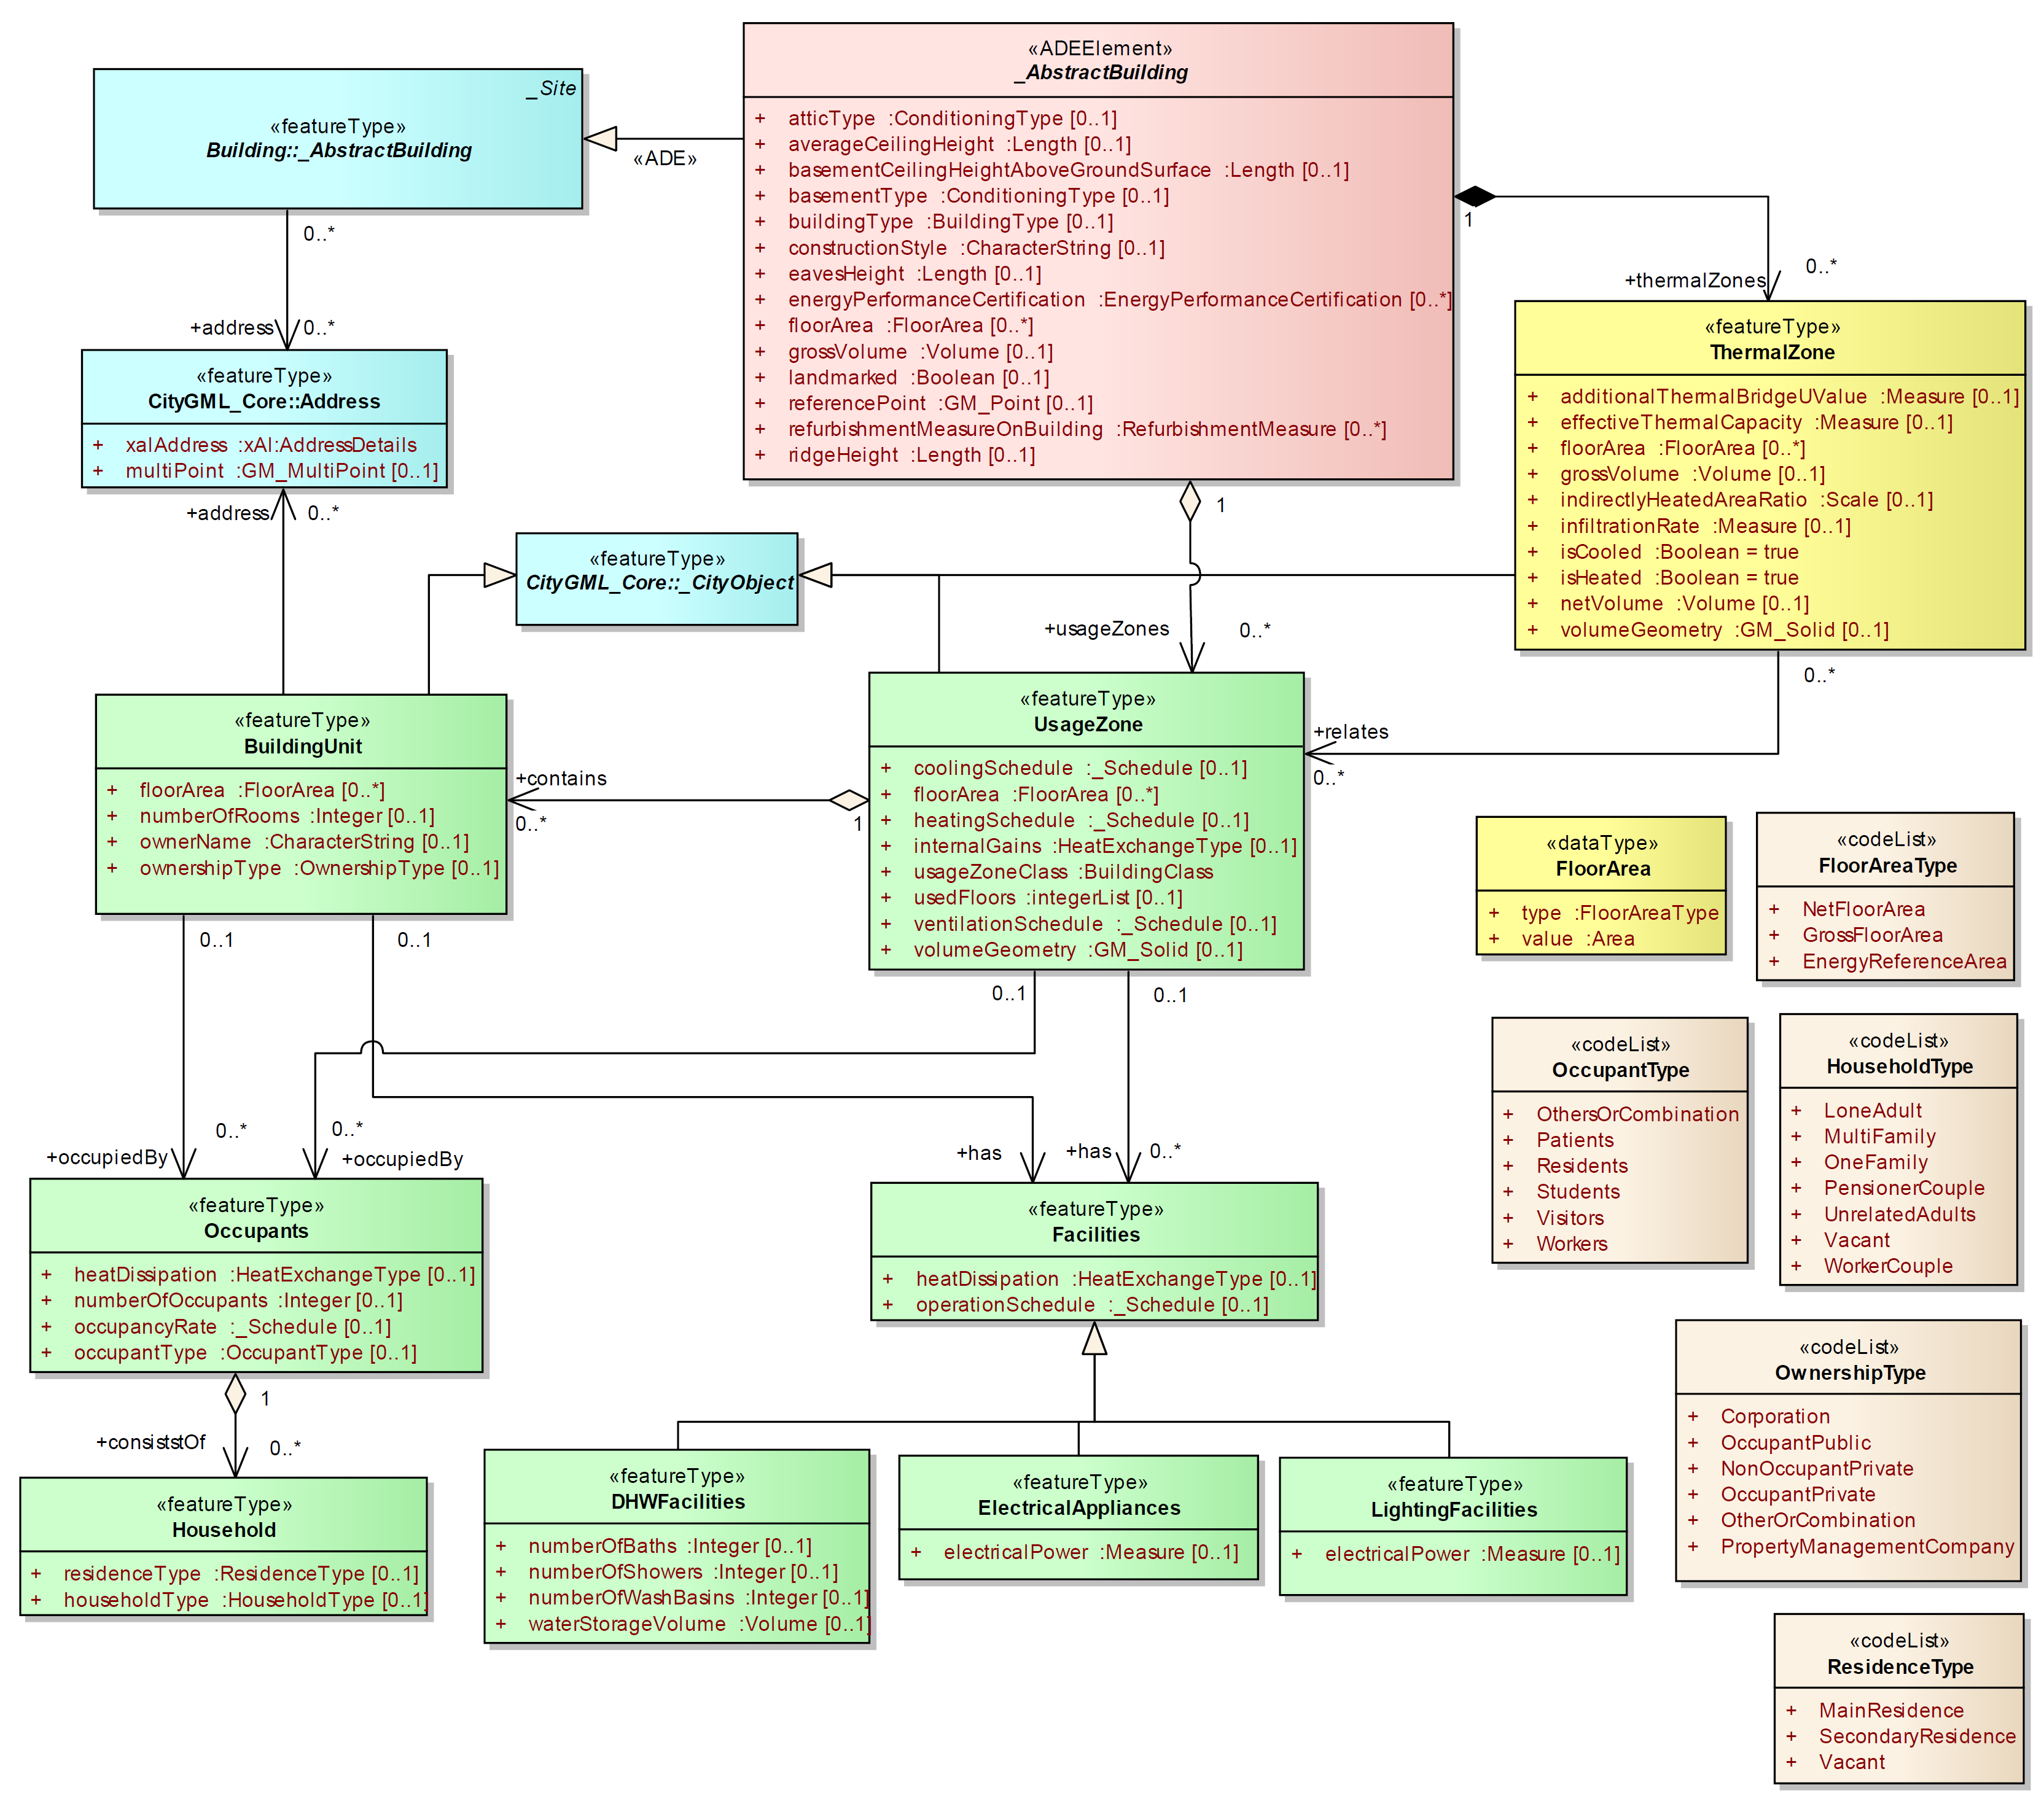
\includegraphics{fig/class_occupancy.png}
\caption{Class diagram of Occupancy Module}
\end{figure}

The Occupancy Module is a module of the ADE Energy, which may be
extended for multi-field analysis (socio-economics, demographics etc.).
It contains the characterization of the building usage, it is related to
the rest of the ADE Energy and CityGML model through the unique class
\texttt{UsageZone}.

\subsection{Usage zone and Building
Unit}\label{usage-zone-and-building-unit}

\subsubsection{UsageZone}\label{usagezone}

Zone of a building with homogeneous usage type. It is a semantic object,
with an optional geometry (\texttt{volumeGeometry}), which may be or not
related to a geometric entity (Building, BuildingPart, Room etc.).

Its usage type is defined by a \texttt{usageZoneClass} (corresponding to
the CityGML Code list of the \texttt{\_AbstractBuilding} attribute
class). This zone is operated with a single heating and cooling
set-point temperature schedule (\texttt{heatingSchedule} respectively
\texttt{coolingSchedule}) and single air ventilation schedule.

This class inherits from \texttt{\_CityObject}, and may therefore be
associated to 1 or more `EnergyDemand' objects. This class is defined
minimally by a usage zone class and a floor area. The building storeys
occupied by this UsageZone may be also indicated
(\texttt{usedFloorNumbers}), 0 corresponding to the ground floor.

Its \texttt{internalGains} attribute correspond to the sum of the energy
dissipated from the occupants and the facilities inside the zone.

\subsubsection{BuildingUnit}\label{buildingunit}

Part of usage zone which is related to a single occupant entity, such as
dwelling or workplace. Owner information data (as owner name and
ownership type) are specified in this class.

It inherits from \texttt{\_CityObject}.

\subsection{Occupants}\label{occupants}

Homogeneous group of occupants of a usage zone or building unit, defined
with an occupant type (e.g.~residents, workers, visitors etc.).

\subsection{Household}\label{household}

Group of persons living in the same dwelling, in the case where
occupants are residents.

There are defined by a type (e.g.~one family, worker couple etc\ldots{})
and a residence type (main/secondary residence or vacant).

\subsection{Facilities}\label{facilities}

Facilities and Appliances inside the usage zone or building unit, which
consume and dissipate energy, without having for first purpose to
regulate the zone thermal comfort. They are distinguished between
domestic hot water (\texttt{DHWFacilities}), specific electrical
appliances (\texttt{ElectricalAppliances}) and lighting facilities
(\texttt{LightingFacilities}). HVAC systems do not belong to these
categories, they are part of the Energy System Module.

\subsubsection{DHWFacilities}\label{dhwfacilities}

\subsubsection{ElectricalAppliances}\label{electricalappliances}

\subsubsection{LightingFacilities}\label{lightingfacilities}

\section{Energy System Module}\label{energy-system-module}

\begin{figure}[htbp]
\centering
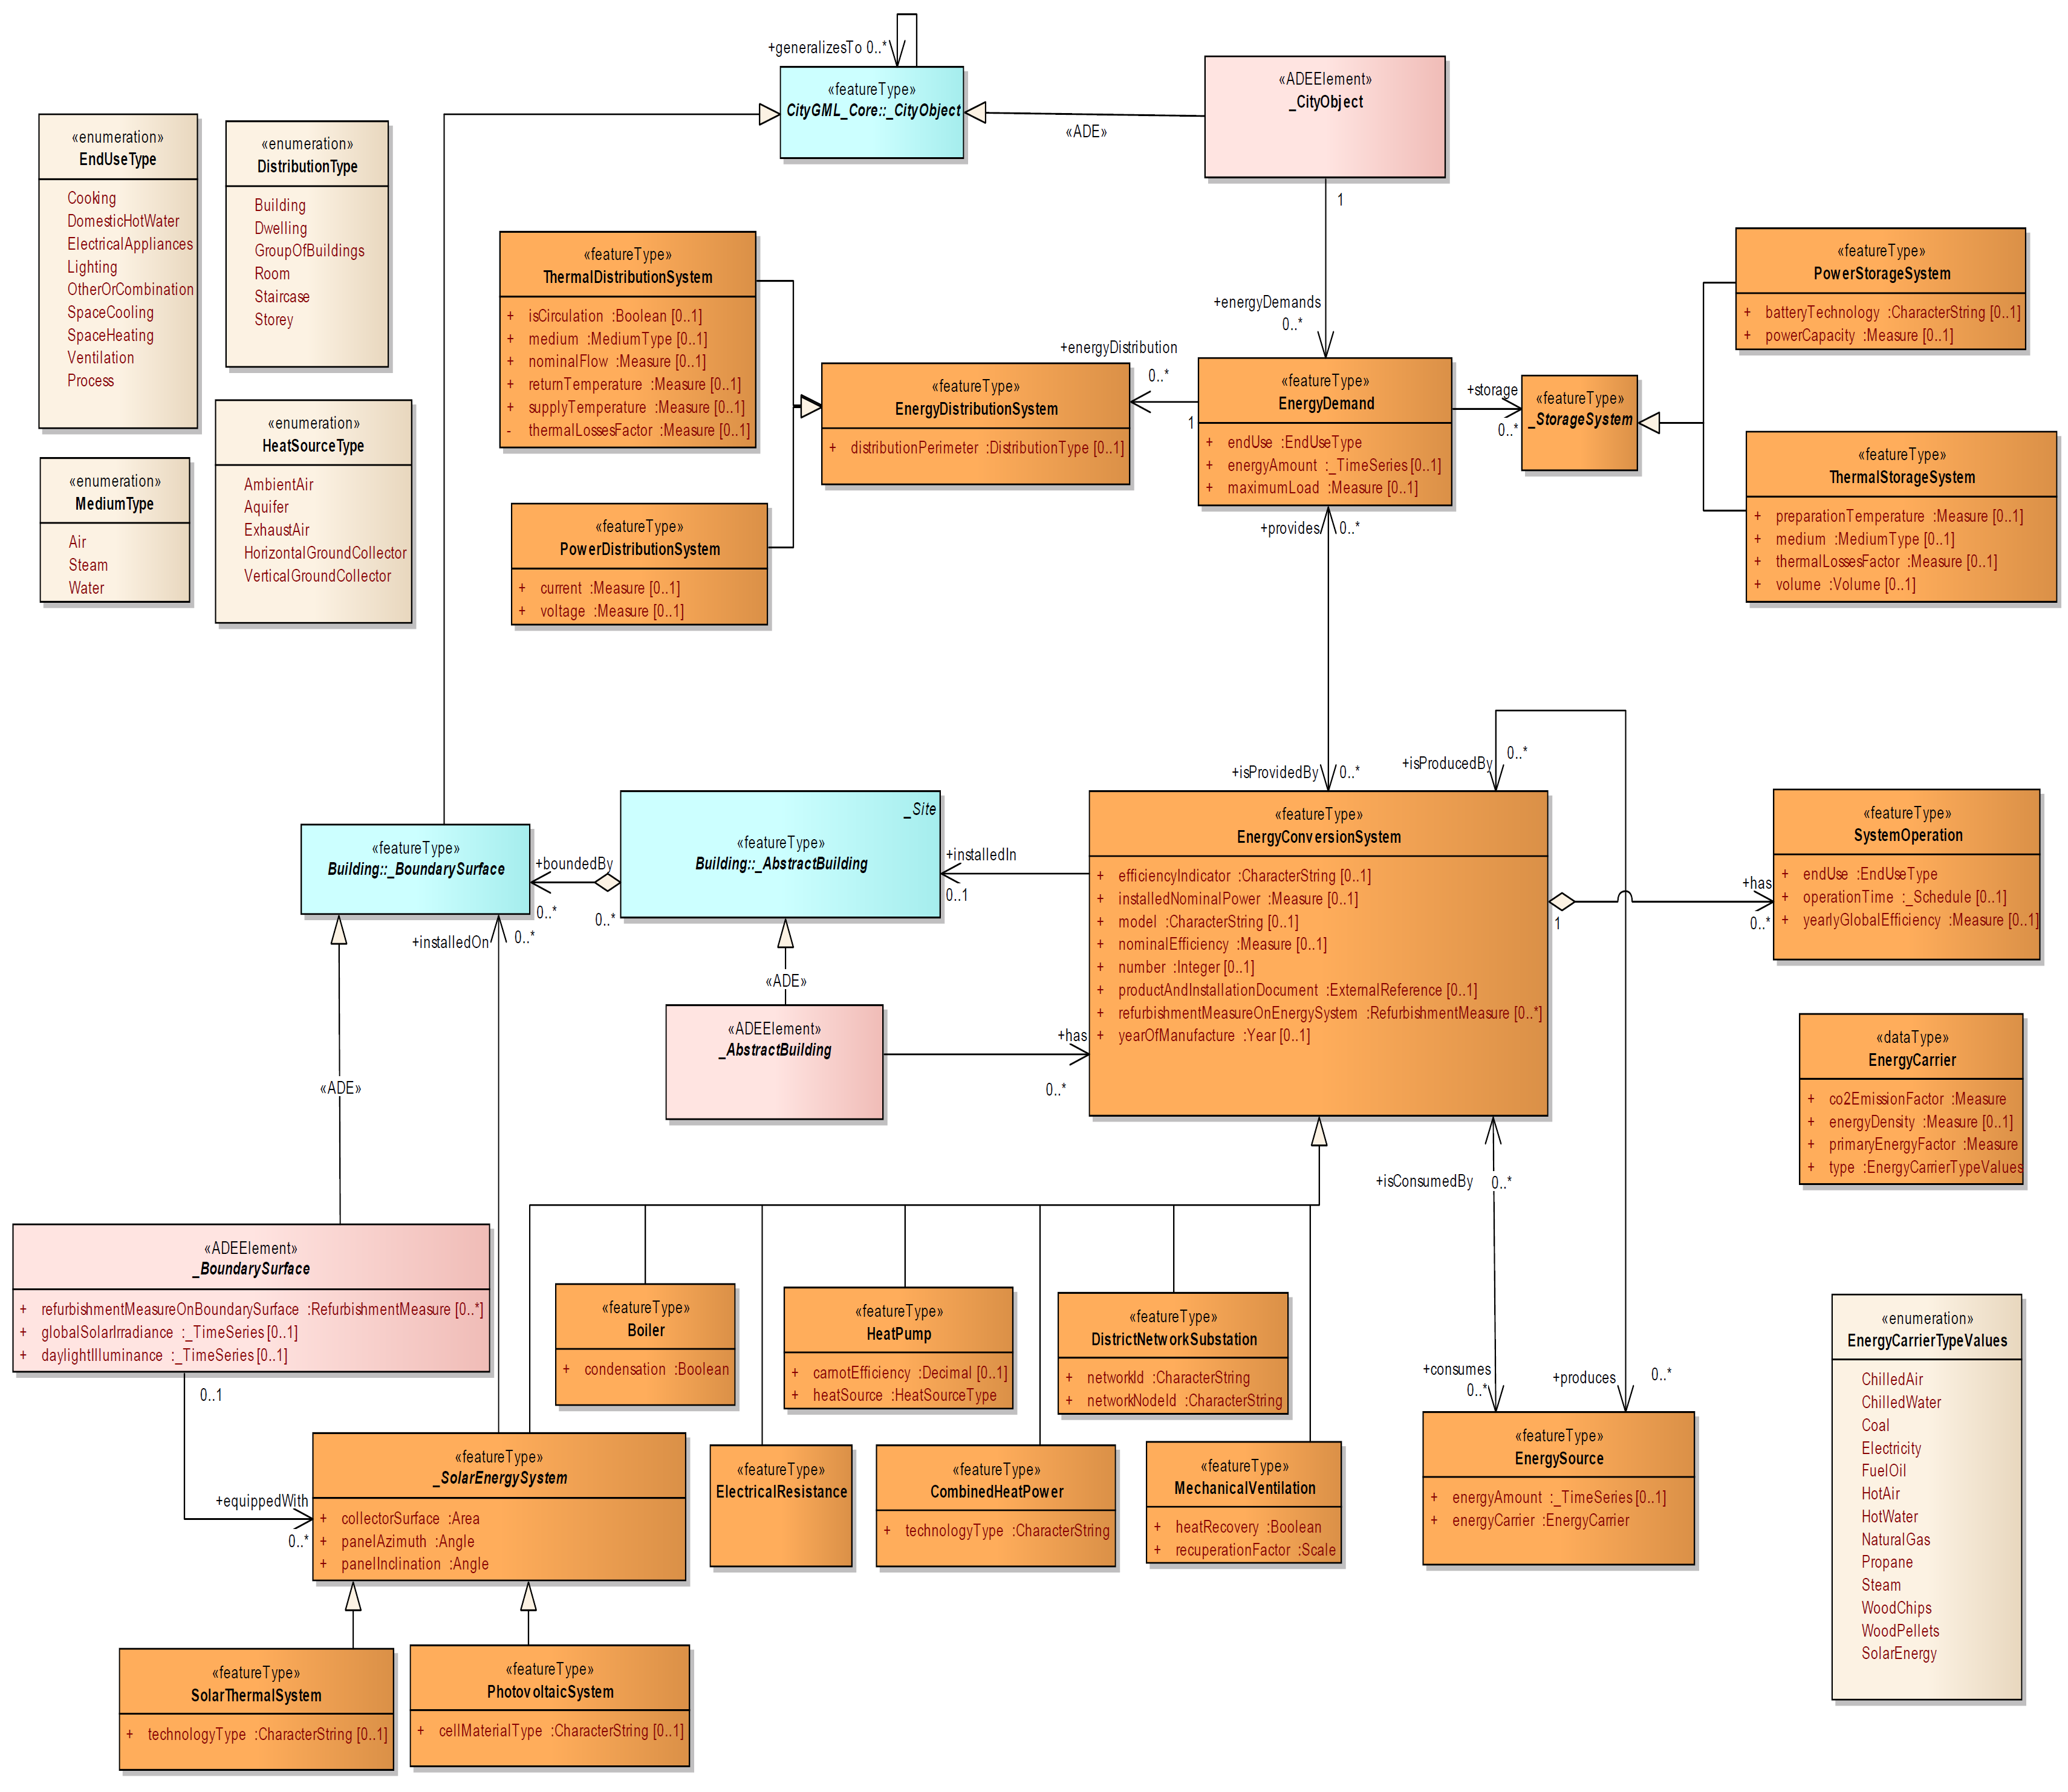
\includegraphics{fig/class_EnergySystem.png}
\caption{Class diagram of Energy System Module}
\end{figure}

The Energy System Module is a module of the ADE Energy, which contains
the information concerning the energy forms (energy demand, supply,
sources) and the energy systems (conversion, distribution and storage
systems). It is arranged around one central \texttt{EnergyDemand}
object.

\subsection{Energy Amounts and Forms}\label{energy-amounts-and-forms}

\subsubsection{EnergyDemand}\label{energydemand}

Useful energy required to satisfy a specific end use, such as heating,
cooling, domestic hot water etc. Beside its \texttt{EndUseType}, this
object is characterized its \texttt{energyAmount} (time-depending energy
demand value) and its maximum yearly load (\texttt{maximumLoad}) used
for the sizing of the energy systems.

Every \texttt{\_CityObject} (typically \texttt{ADE:\_AbstractBuilding},
\texttt{ThermalZone}, \texttt{UsageZone} and \texttt{BuildingUnit}) may
have one or more \texttt{EnergyDemand}.

\subsubsection{EndUseType}\label{endusetype}

List of possible end uses as cooking, space heating and ventilation.

\subsubsection{EnergySource}\label{energysource}

Final energy consumed (and sometimes produced) by the energy conversion
system.

Its energy characteristics are specified in the Energy Carrier object.

\subsubsection{EnergyCarrier}\label{energycarrier}

Primary energy and \(CO_2\) emission factors, energy density and energy
carrier type characterize this data type for energy carriers.

\subsubsection{EnergyCarrierType}\label{energycarriertype}

List of energy carriers as coal, chilled water or electricity.

\subsection{Energy Distribution}\label{energy-distribution}

\subsubsection{EnergyDistributionSystem}\label{energydistributionsystem}

System in charge of delivering the energy inside the building, from the
place of energy production to the place of end-use. Power and Thermal
distribution systems are differentiated. They all share a distribution
perimeter that is described by the distribution type.

\subsubsection{Distribution Type}\label{distribution-type}

A list of possible distribution perimeters, e.g.~Building, Dwelling,
Room.

\subsubsection{ThermalDistributionSystem}\label{thermaldistributionsystem}

Type for thermal distribution systems with attributes for circulation
(circulating system or not), the used medium, nominal flow, return and
supply temperatures and thermal losses factor.

\subsubsection{PowerDistributionSystem}\label{powerdistributionsystem}

Type for electrical distribution systems, described by current and
voltage.

\subsubsection{MediumType}\label{mediumtype}

This list is a collection of medium types as air and water.

\subsection{Energy Storage}\label{energy-storage}

\subsubsection{StorageSystem}\label{storagesystem}

System storing energy. A same storage may store the energy of different
end-users and different end uses. Power and Thermal storage systems are
differentiated.

\subsubsection{ThermalStorageSystem}\label{thermalstoragesystem}

Thermal storages with a medium, preparation temperature, thermal losses
factor and a volume.

\subsubsection{PowerStorageSystem}\label{powerstoragesystem}

Electrical storages with an electrical capacity and a string to describe
the battery technology.

\subsection{Energy Conversion}\label{energy-conversion}

\subsubsection{EnergyConversionSystem}\label{energyconversionsystem}

System converting an energy source into the energy necessary to satisfy
the \texttt{EnergyDemand} (or to feed the networks).

Energy conversion systems have common parameters: efficiency indicator,
nominal installed power, nominal efficiency (in reference to an
efficiency indicator), year of manufacture, name of the model, a serial
number, a reference to product or installation documents and optionally
refurbishment measures. They may be one or more (in this case, the
nominal installed power corresponds to the totality).

Specific energy conversion systems may have in addition specific
parameters:

A same system may have several operation modes (e.g.~heat pump covering
heating and domestic hot water demands).

\subsubsection{SystemOperation}\label{systemoperation}

It details the operation of the energy conversion system for a specific
end-use and operation time. For instance, a reversible heat pump may
have 3 operation modes: heating production in winter, cooling production
in summer, and hot water production during the whole year. Attributes
are end use type, a schedule for operation time and yearly global
efficiency.

\subsubsection{DistrictNetworkSubstation}\label{districtnetworksubstation}

Subtype of \texttt{EnergyConversionSystem} for heating or cooling
networks substations. Adds attributes for network ID and network node
ID.

\subsubsection{HeatPump}\label{heatpump}

Subtype of \texttt{EnergyConversionSystem} for heat pumps to add carnot
efficiency and heat source. Heat source is described using a
\texttt{HeatSourceType}.

\subsubsection{HeatSourceType}\label{heatsourcetype}

List of heat source types for heat pumps, e.g.~ambient air, aquifer and
exhaust air.

\subsubsection{ElectricalResistance}\label{electricalresistance}

Subtype of \texttt{EnergyConversionSystem} for electrical resistances.
Comes without additional attributes.

\subsubsection{MechanicalVentilation}\label{mechanicalventilation}

Subtype of \texttt{EnergyConversionSystem} for ventilation systems with
attributes heat recovery (with or without) and recuperation factor.

\subsubsection{CombinedHeatPower}\label{combinedheatpower}

Subtype of \texttt{EnergyConversionSystem} for CHP systems. Utilizes a
string describing the technology type.

\subsubsection{Boiler}\label{boiler}

Subtype of \texttt{EnergyConversionSystem} for boiler. Defines if it is
a condensation boiler or not.

\subsubsection{SolarEnergySystem}\label{solarenergysystem}

Subclass of \texttt{EnergyConversionSystem} for solar energy systems.
Has attributes for collector surface, azimuth and inclination.
Differentiates into solar thermal and photovoltaic systems.

\subsubsection{SolarThermalSystem}\label{solarthermalsystem}

Subtype of \texttt{SolarEnergySystem} for thermal systems. Uses a string
to describe the technology type.

\subsubsection{PhotovoltaicSystem}\label{photovoltaicsystem}

Subtype of \texttt{SolarEnergySystem} for photovoltaic systems. Defines
the material type of photovoltaic cells with a string.

\section*{References}\label{references}
\addcontentsline{toc}{section}{References}

\hypertarget{refs}{}

\end{document}
